\section{Démonstration contrôlée : 25 modèles, un seul protocole}\label{sec:demo}

Les sections précédentes décrivent des runs qui changeaient plusieurs choses à la fois. Le notebook \code{v\_demo/CFM\_demo\_models} reprend le projet de zéro, avec des modèles volontairement simples (chacun moins de 20 minutes sur GPU) et un protocole \emph{identique} pour tous : même cache, mêmes partitions (fit, valid par grappes de régime, stress = carnets les moins profonds), mêmes métriques. Son but n'est pas de battre le LB. Il sert à \emph{attribuer} chaque gain à une seule cause. Toutes les mesures sont internes, sans pseudo-labels, donc sans la contamination de la section~\ref{sec:contam}.

\begin{figure}[H]\centering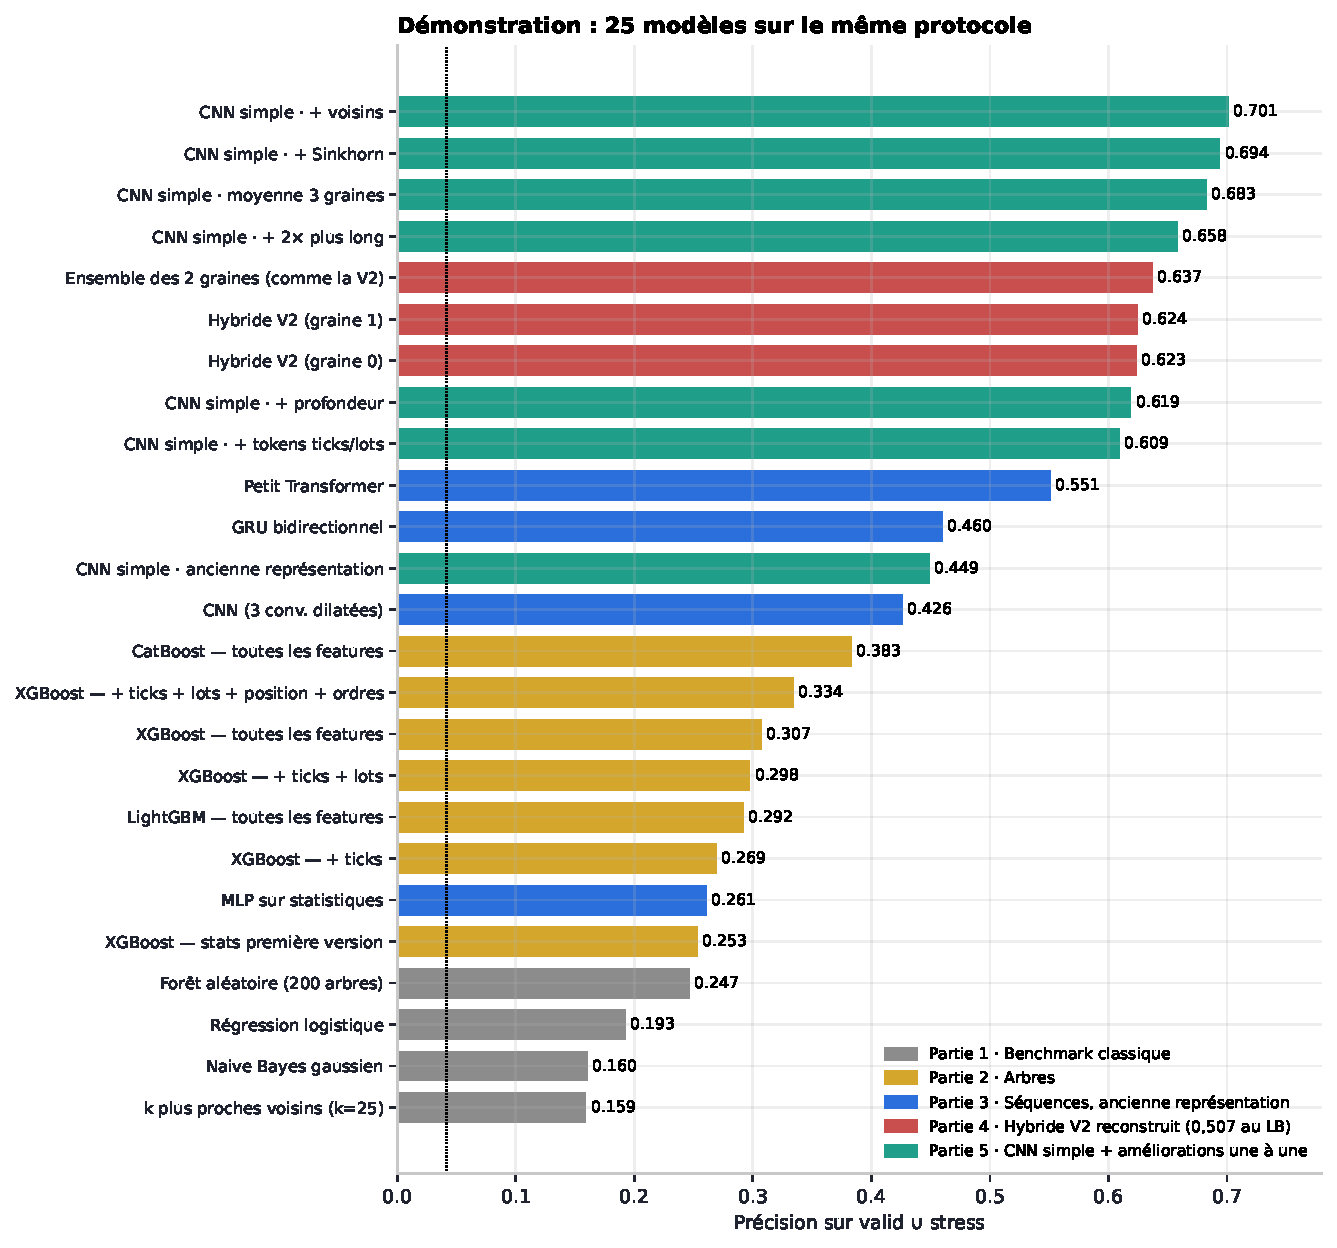
\includegraphics[width=.86\linewidth]{figures/demo_synthese.pdf}
\caption{Les 25 modèles du notebook, classés par précision sur valid $\cup$ stress. Pour les parties 1 à 4, c'est la moyenne pondérée des précisions équilibrées valid et stress. Pour la partie 5, c'est la précision mesurée directement sur l'union (équilibrée à partir de l'étape Sinkhorn). Un petit CNN d'environ 100\,k paramètres, nourri des tokens en ticks et en lots, dépasse la reconstruction de l'ancien meilleur modèle dès qu'on l'entraîne plus longtemps.}
\label{fig:demo-synth}\end{figure}

\subsection{Parties 1 et 2 : modèles classiques et arbres}
\begin{figure}[H]\centering
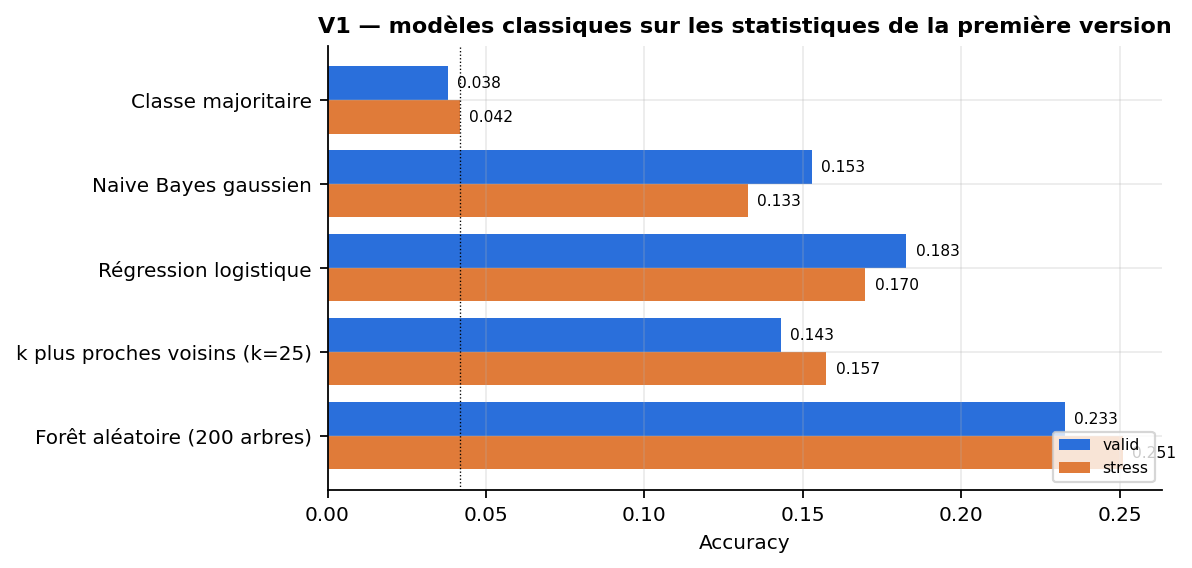
\includegraphics[width=.49\linewidth]{figures/demo_v1_compare.png}\hfill
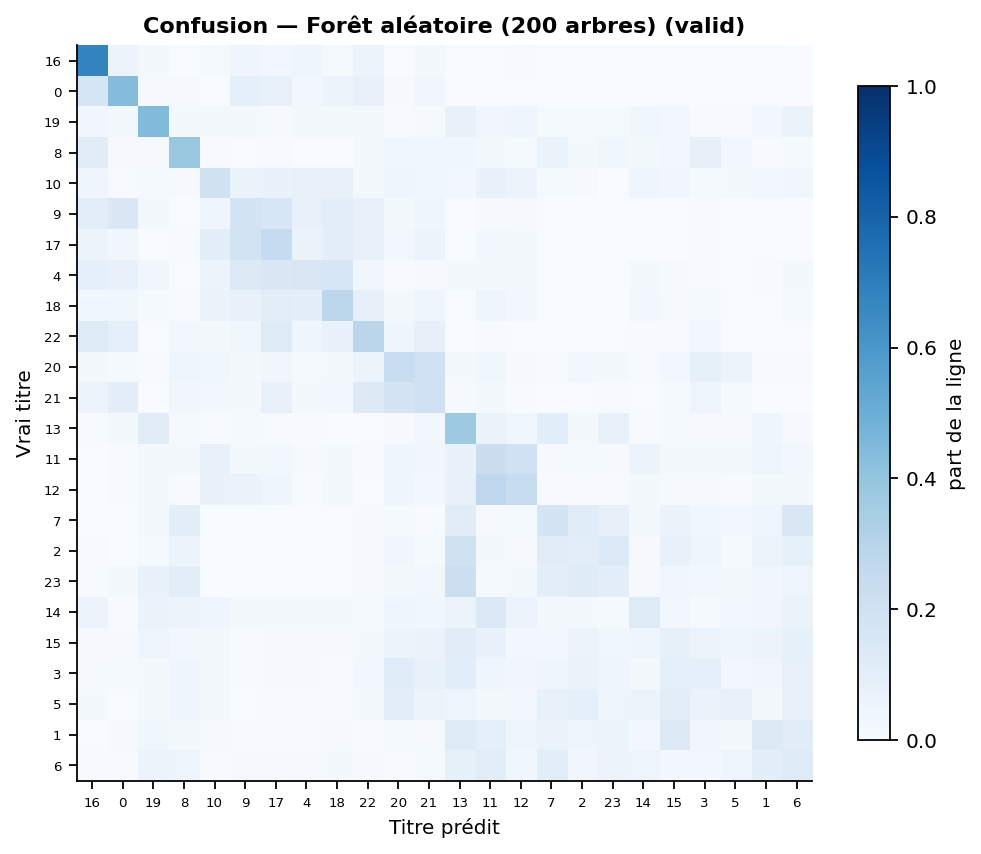
\includegraphics[width=.44\linewidth]{figures/demo_v1_confusion.png}
\caption{Partie 1. Modèles classiques sur les statistiques de fenêtre de la toute première version. Le meilleur, une forêt aléatoire, plafonne à 0,23 en valid et 0,25 en stress, avec une confusion diffuse : ces statistiques ne portent presque pas la signature des titres.}
\end{figure}

\begin{figure}[H]\centering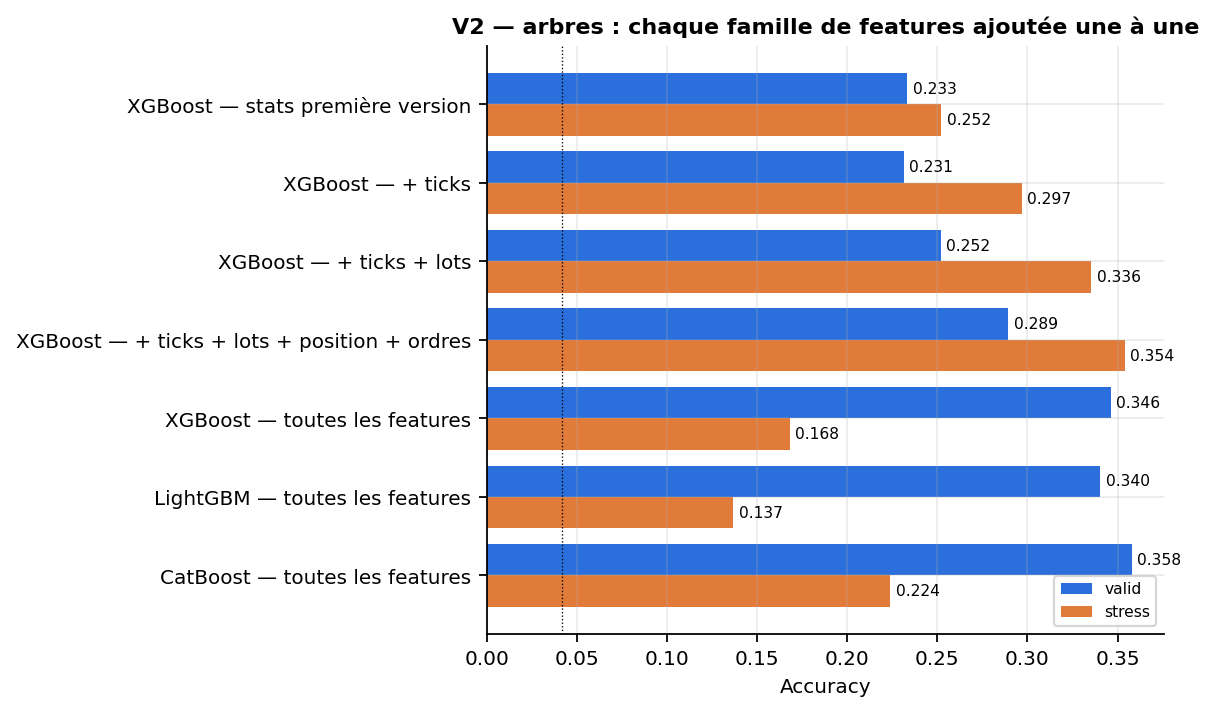
\includegraphics[width=.75\linewidth]{figures/demo_v2_compare.png}
\caption{Partie 2. XGBoost en ajoutant une famille de features à la fois. Les familles stables font monter le \emph{stress} à chaque ajout : 0,252 (statistiques initiales), 0,297 (+ ticks), 0,336 (+ lots), 0,354 (+ position et ordres). Avec \emph{toutes} les features, profondeur comprise, la valid monte à 0,346 mais le stress s'effondre à 0,168 (0,137 pour LightGBM, 0,224 pour CatBoost). C'est le piège de régime de la section~\ref{sec:screening}, reproduit ici sur trois implémentations différentes.}
\label{fig:demo-trees}\end{figure}

\begin{figure}[H]\centering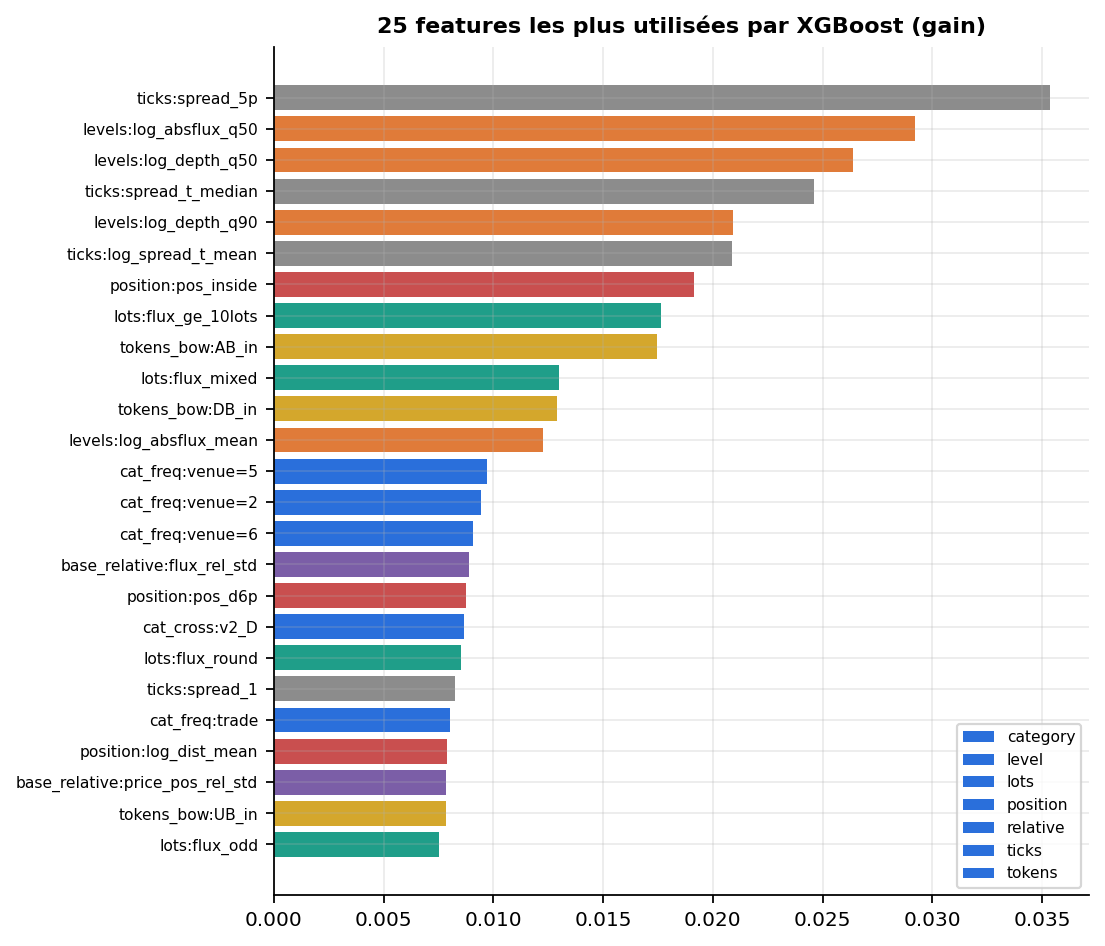
\includegraphics[width=.7\linewidth]{figures/demo_v2_importance.png}
\caption{Les 25 features les plus utilisées par XGBoost (gain). En tête, le spread en ticks (\code{ticks:spread\_5p}), la signature stable, mais juste derrière, trois mesures de profondeur. Un arbre exploite tout ce qui sépare sur la période d'entraînement, sans distinguer signature et régime : c'est exactement ce que la figure~\ref{fig:demo-trees} fait payer en stress.}
\end{figure}

\subsection{Parties 3 et 4 : lire la séquence, et l'ancien record}
\begin{figure}[H]\centering
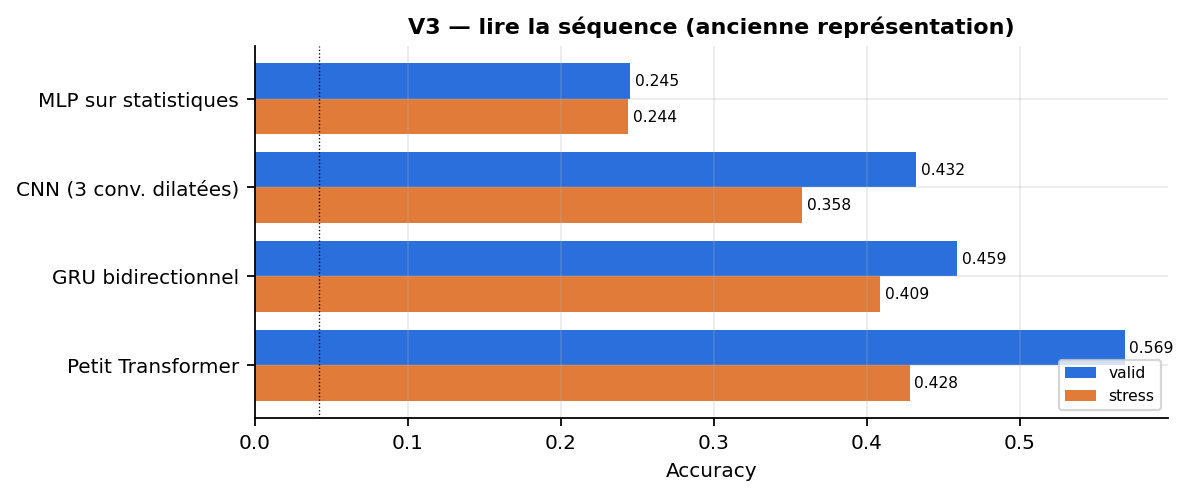
\includegraphics[width=.47\linewidth]{figures/demo_v3_compare.png}\hfill
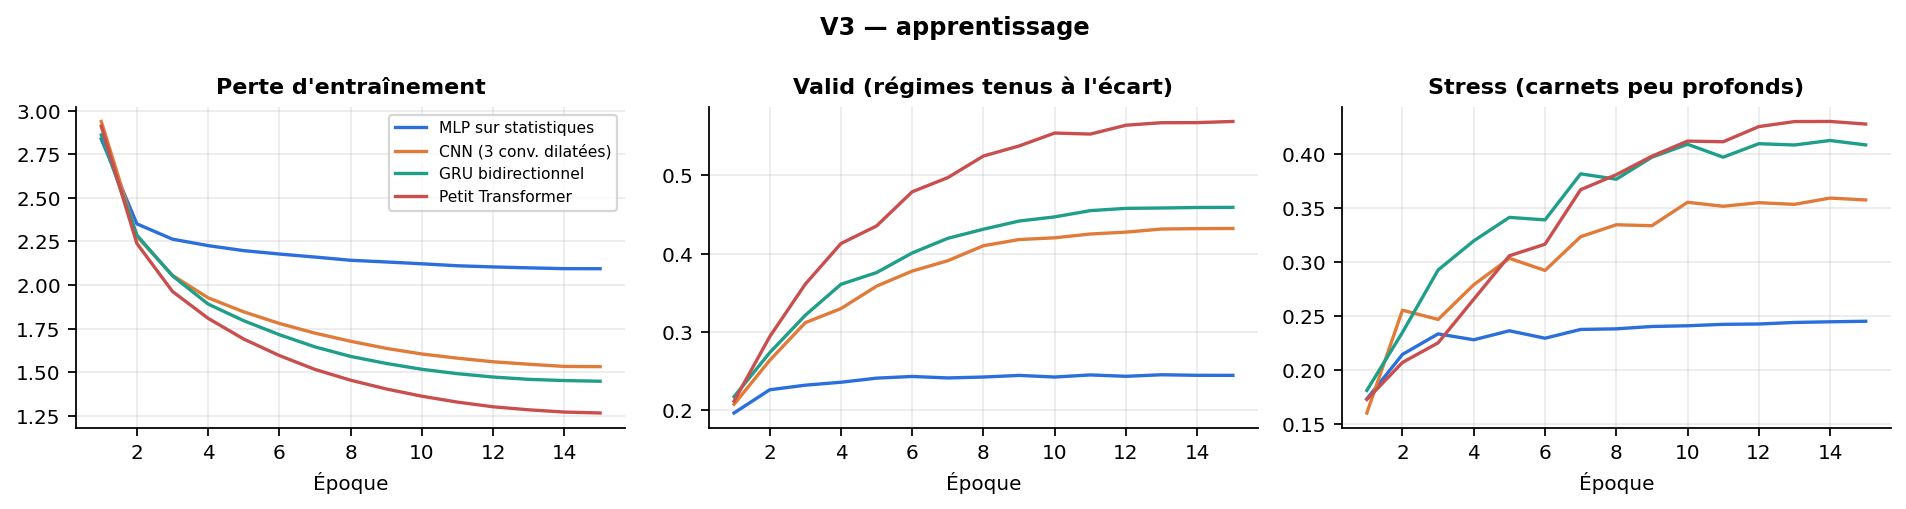
\includegraphics[width=.51\linewidth]{figures/demo_v3_curves.png}
\caption{Partie 3. Quatre réseaux sur l'\emph{ancienne} représentation relative. Lire la séquence plutôt que des résumés fait passer la valid de 0,245 (MLP sur statistiques) à 0,432 (CNN), 0,459 (GRU bidirectionnel) et 0,569 (petit Transformer). Même avec de mauvaises unités, l'ordre des événements porte beaucoup d'information.}
\end{figure}

\begin{figure}[H]\centering
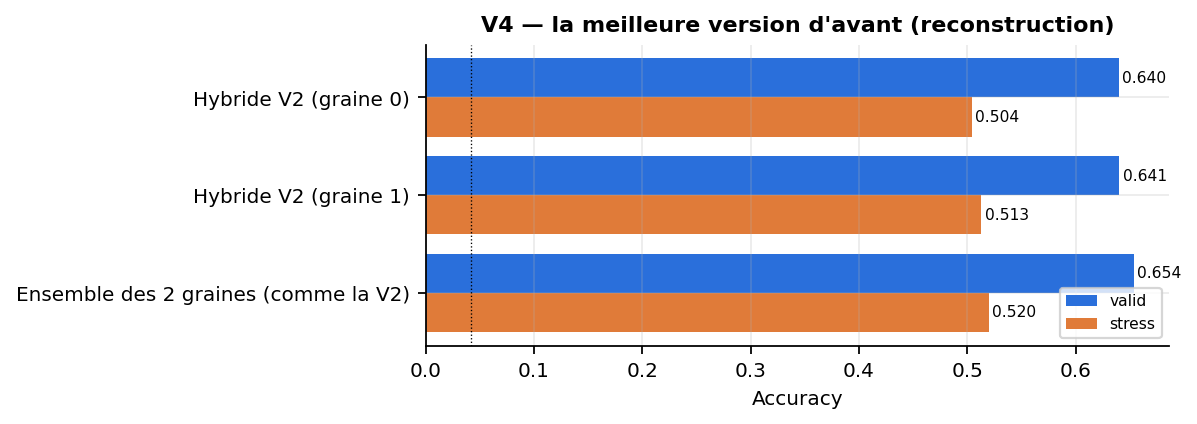
\includegraphics[width=.47\linewidth]{figures/demo_v4_compare.png}\hfill
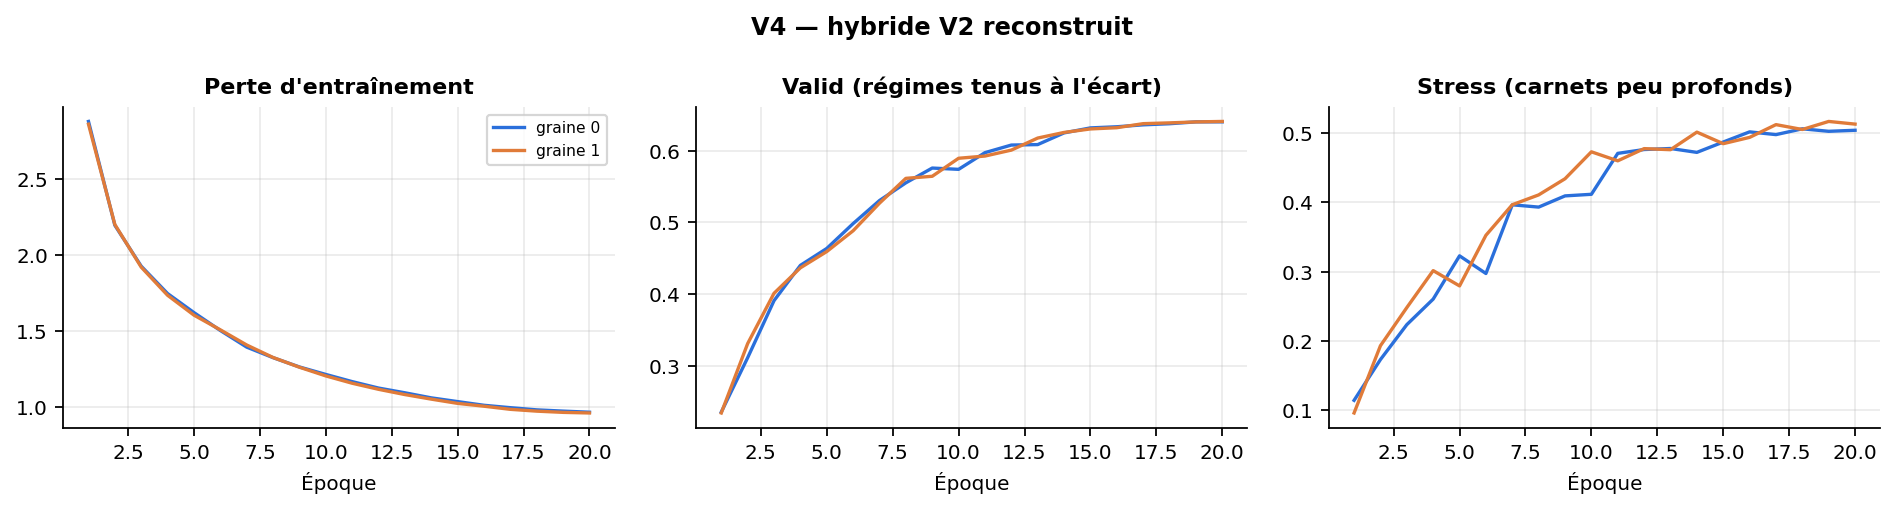
\includegraphics[width=.51\linewidth]{figures/demo_v4_curves.png}
\caption{Partie 4. Reconstruction simplifiée du Transformer hybride de la V2, le record historique à 0,507 au LB. Deux graines donnent 0,640--0,641 en valid et 0,504--0,513 en stress, l'ensemble 0,654 et 0,520. Fait notable : le stress brut de ce modèle (0,52) est très proche de son score public (0,507), alors que la valid le surestime de 15 points.}
\label{fig:demo-v2}\end{figure}

\subsection{Partie 5 : les améliorations, une à la fois}
On part d'un petit CNN (trois convolutions dilatées, environ 100\,k paramètres) qui lit l'ancienne représentation, puis on ajoute \emph{une seule} chose à chaque étape, toujours mesurée sur les mêmes 42\,627 fenêtres de valid $\cup$ stress.

\begin{table}[H]\centering\small
\begin{tabular}{clcc}
\toprule
Étape & Ajout & Précision valid $\cup$ stress & Gain\\
\midrule
0 & ancienne représentation (20 époques) & 0,449 & —\\
1 & \textbf{tokens en ticks et en lots} & 0,609 & \textbf{+16,0}\\
2 & augmentation de profondeur ($\sigma=0{,}3$) & 0,619 & +1,0\\
3 & entraînement deux fois plus long (40 époques) & 0,658 & +3,9\\
4 & moyenne de 3 graines & 0,683 & +2,5\\
5 & équilibrage de Sinkhorn & 0,694 & +1,1\\
6 & vote entre voisins (\code{combo}, $k=10$, $\alpha=0{,}5$, 5 it.) & \textbf{0,701} & +0,7\\
\bottomrule
\end{tabular}
\caption{L'échelle de la partie 5. Les étapes 5 et 6 n'utilisent que le pool lui-même (voisins cherchés dans valid $\cup$ stress), sans le test.}
\label{tab:ladder}\end{table}

\begin{figure}[H]\centering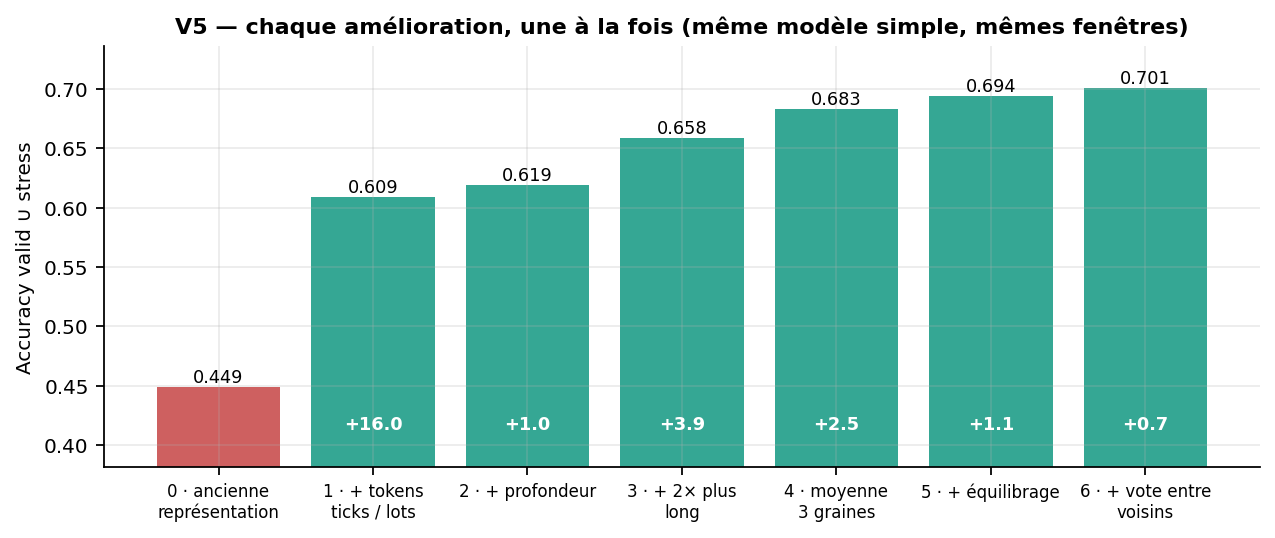
\includegraphics[width=.85\linewidth]{figures/demo_v5_ladder.png}
\caption{L'échelle de la table~\ref{tab:ladder} en image. À comparer avec la progression publique de la figure~\ref{fig:lb} : les leviers arrivent dans le même ordre d'importance, à une exception près. Le vote entre voisins rapporte peu en interne (+0,7) et beaucoup au LB (+3,2), parce que le test contient quatre fois plus de fenêtres par titre-jour que le pool.}
\end{figure}

\paragraph{Ce que l'échelle établit.} La section~\ref{sec:limites} notait que les $+6{,}3$ points du premier run mêlaient représentation, architecture et ensemble. L'étape 1 isole la représentation : \emph{même} réseau, \emph{même} entraînement, \emph{mêmes} fenêtres. Passer de l'ancienne représentation relative aux tokens en ticks et en lots vaut à elle seule \textbf{+16 points} internes, plus que toutes les autres étapes réunies (+9,2). C'est la mesure la plus nette du projet en faveur de la thèse des unités naturelles. Elle reste interne : son ampleur au LB n'est pas mesurée.

\begin{figure}[H]\centering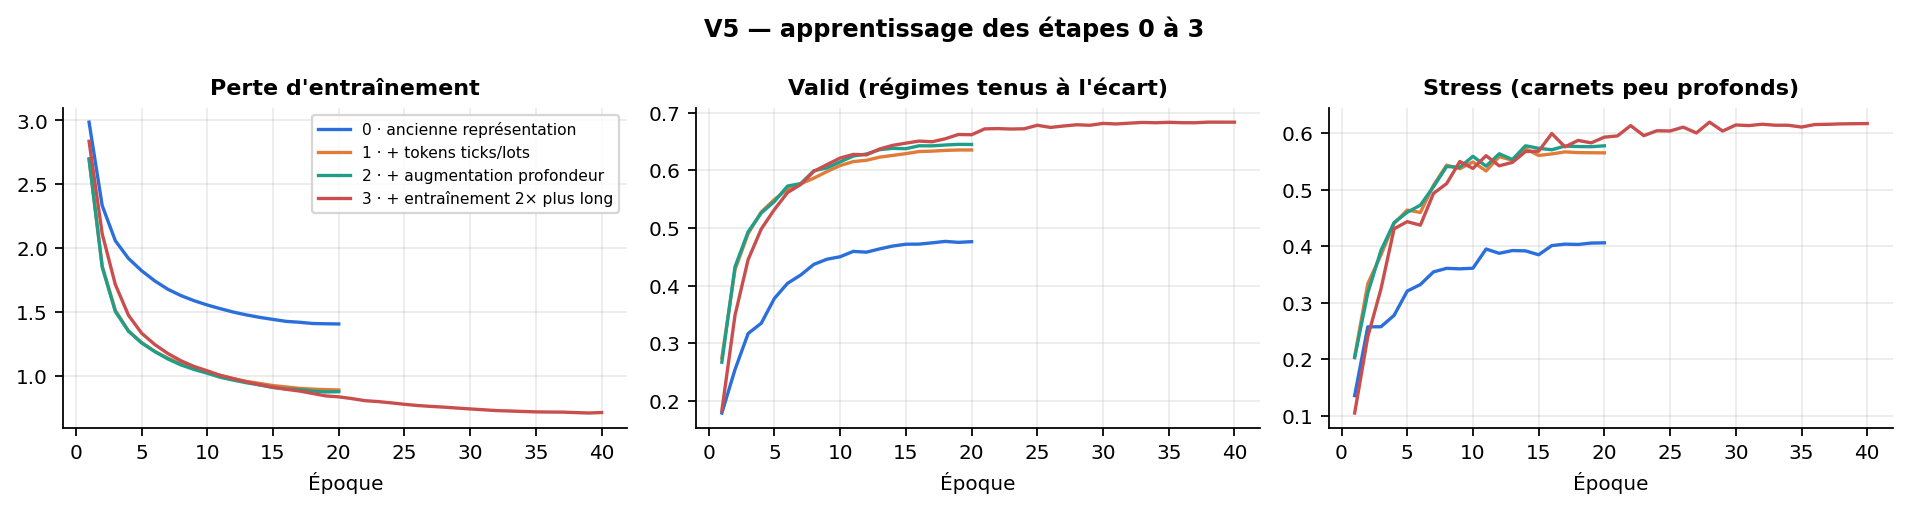
\includegraphics[width=\linewidth]{figures/demo_v5_curves.png}
\caption{Courbes d'apprentissage des étapes 0 à 3. L'ancienne représentation (bleu) plafonne vers 0,47 en valid. Toutes les variantes à tokens montent plus vite et plus haut. L'entraînement long (rouge) continue de progresser jusqu'à l'époque 40.}
\end{figure}

\begin{figure}[H]\centering
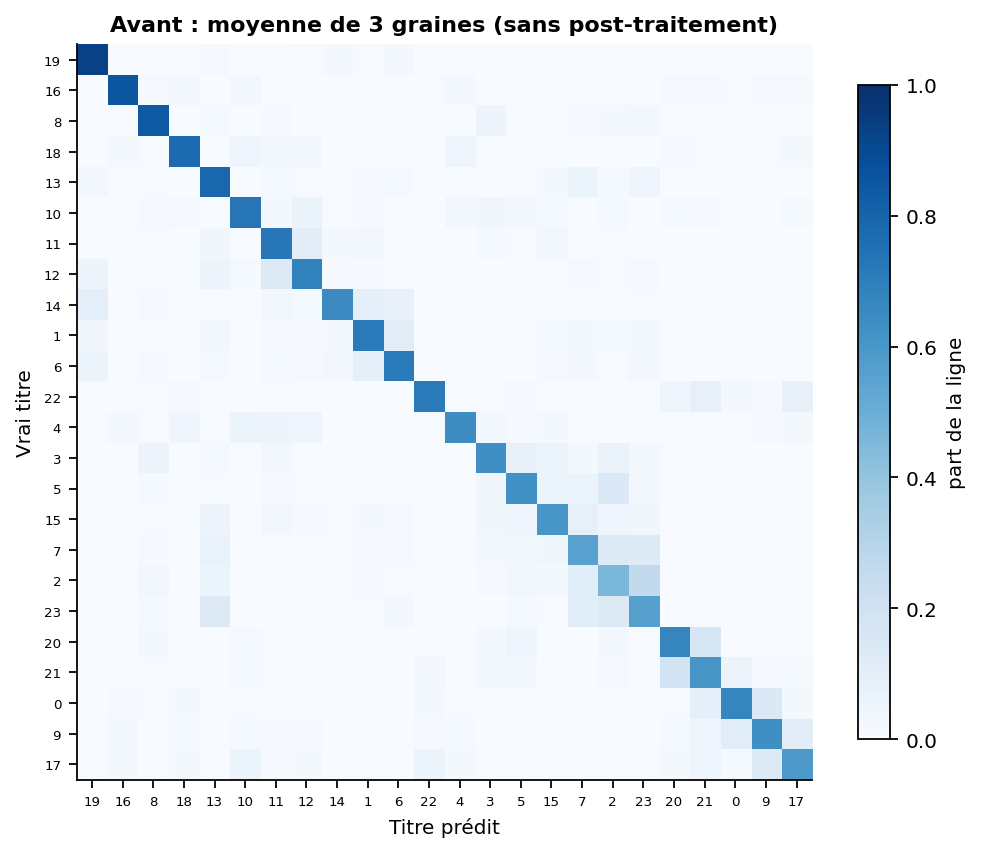
\includegraphics[width=.49\linewidth]{figures/demo_v5_confusion_before.png}\hfill
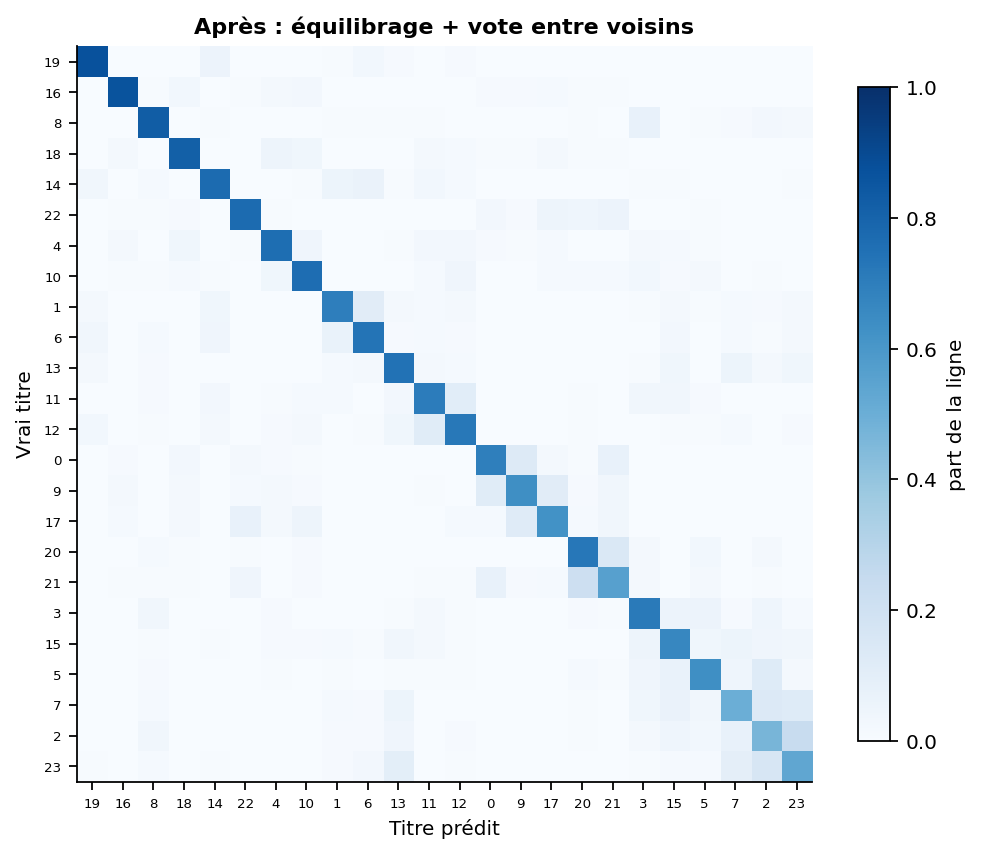
\includegraphics[width=.49\linewidth]{figures/demo_v5_confusion_after.png}
\caption{Confusions du CNN simple sur le stress, avant (moyenne de 3 graines) et après (équilibrage + vote entre voisins). Les erreurs restantes se concentrent dans les mêmes familles que pour le grand modèle, $\{20,21\}$, $\{2,7,23\}$, $\{0,9,17\}$ : elles tiennent à la donnée plus qu'au modèle.}
\end{figure}

\begin{figure}[H]\centering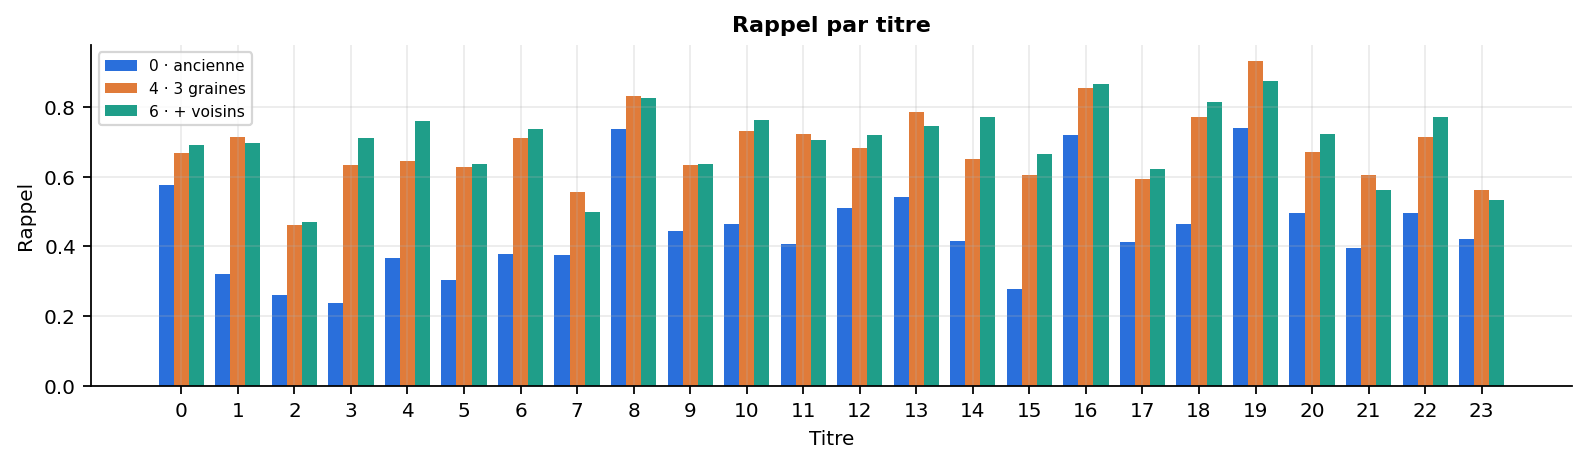
\includegraphics[width=.9\linewidth]{figures/demo_v5_recall.png}
\caption{Rappel par titre : ancienne représentation (étape 0), 3 graines (étape 4), après voisins (étape 6). Le gain est général, il ne vient pas de quelques titres faciles. Les plus gros sauts concernent des titres que l'ancienne représentation ne reconnaissait presque pas (1, 3, 5, 15 : de 0,25--0,3 à plus de 0,6).}
\end{figure}

\begin{figure}[H]\centering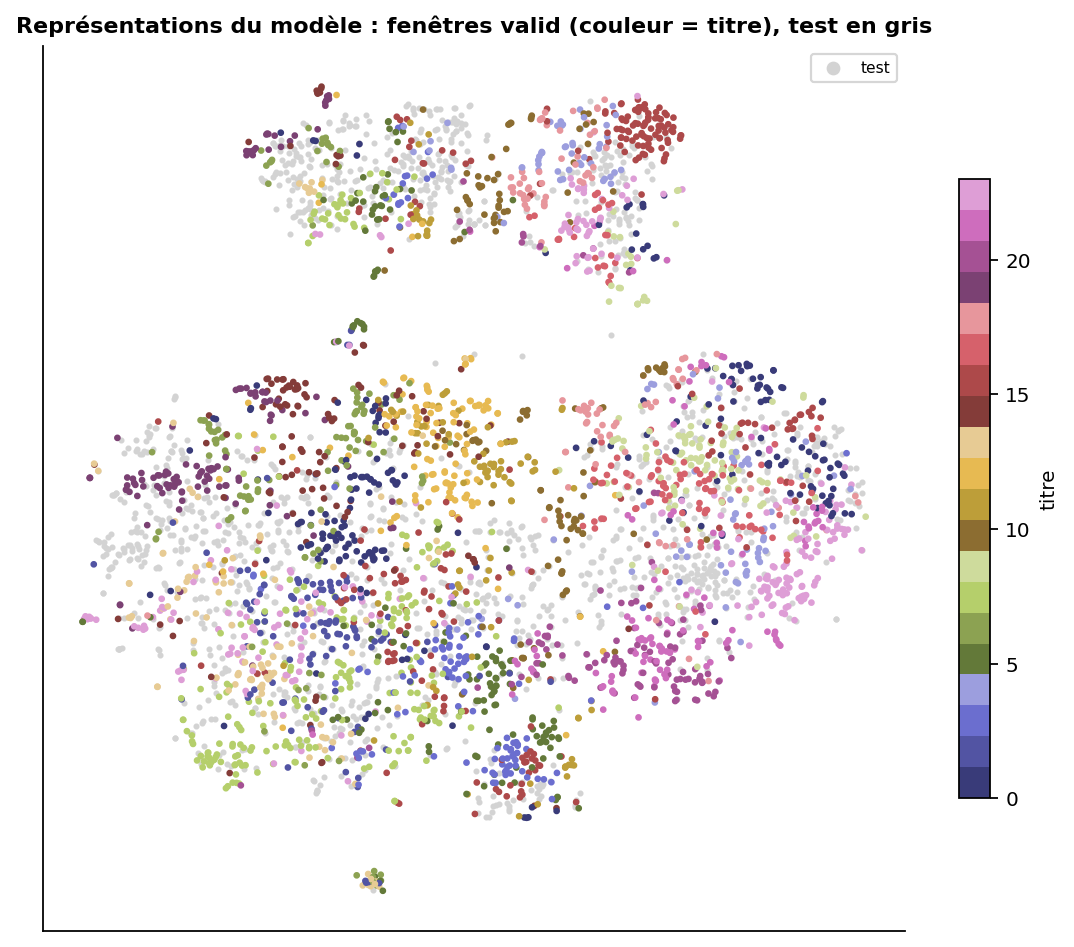
\includegraphics[width=.62\linewidth]{figures/demo_v5_tsne.png}
\caption{Représentations internes du CNN simple (t-SNE) : fenêtres valid colorées par titre, fenêtres test en gris. Le test occupe les mêmes régions que la valid, sans îlot isolé : la représentation transfère d'une période à l'autre, ce qui rend le vote entre voisins et l'auto-apprentissage possibles.}
\end{figure}

\subsection{Ce que la démonstration ajoute}
\begin{enumerate}
\item \textbf{Une attribution propre.} À architecture égale, la représentation vaut +16 points internes. Ce n'était qu'une conjecture dans la section~\ref{sec:resultats}.
\item \textbf{Un modèle simple suffit.} Un CNN de 100\,k paramètres, sans attention, atteint 0,683 avant tout post-traitement, contre 0,637 pour la reconstruction de l'ancien record. L'essentiel du gain tient à la donnée et au protocole, pas à la complexité du réseau.
\item \textbf{Le piège de régime est robuste.} Trois implémentations d'arbres le reproduisent : ajouter les features de profondeur fait gagner en valid et perdre en stress.
\end{enumerate}
